\documentclass{beamer}
\usetheme{Luebeck}
\setbeamercovered{dynamic}
\usepackage{graphicx}
\usepackage{fontspec}
\beamertemplatenavigationsymbolsempty

\title{PGP, GPG, and Enigmail... Oh My!}
\author{Jack Rosenthal}
\date{25 January 2016}
\logo{
\includegraphics[width=30mm]{graphics/lug.pdf}}

\begin{document}

\begin{frame}
    \maketitle
\end{frame}
\logo{}

\begin{frame}
    \frametitle{Pretty Good Privacy}
    \begin{itemize}[<+->]
        \item PGP is a data encryption, decryption, and signing program. It
            follows the OpenPGP standard.
        \item People use PGP to sign, encrypt, and decrypt emails, files,
            folders, and even whole disk partitions.
        \item PGP allows you to specify a recipient to encrypt a message for
            given only their public key, you can even encrypt to multiple
            recipients given only their public keys.
    \end{itemize}
\end{frame}

\begin{frame}
    \frametitle{How it Works}
    \begin{center}
        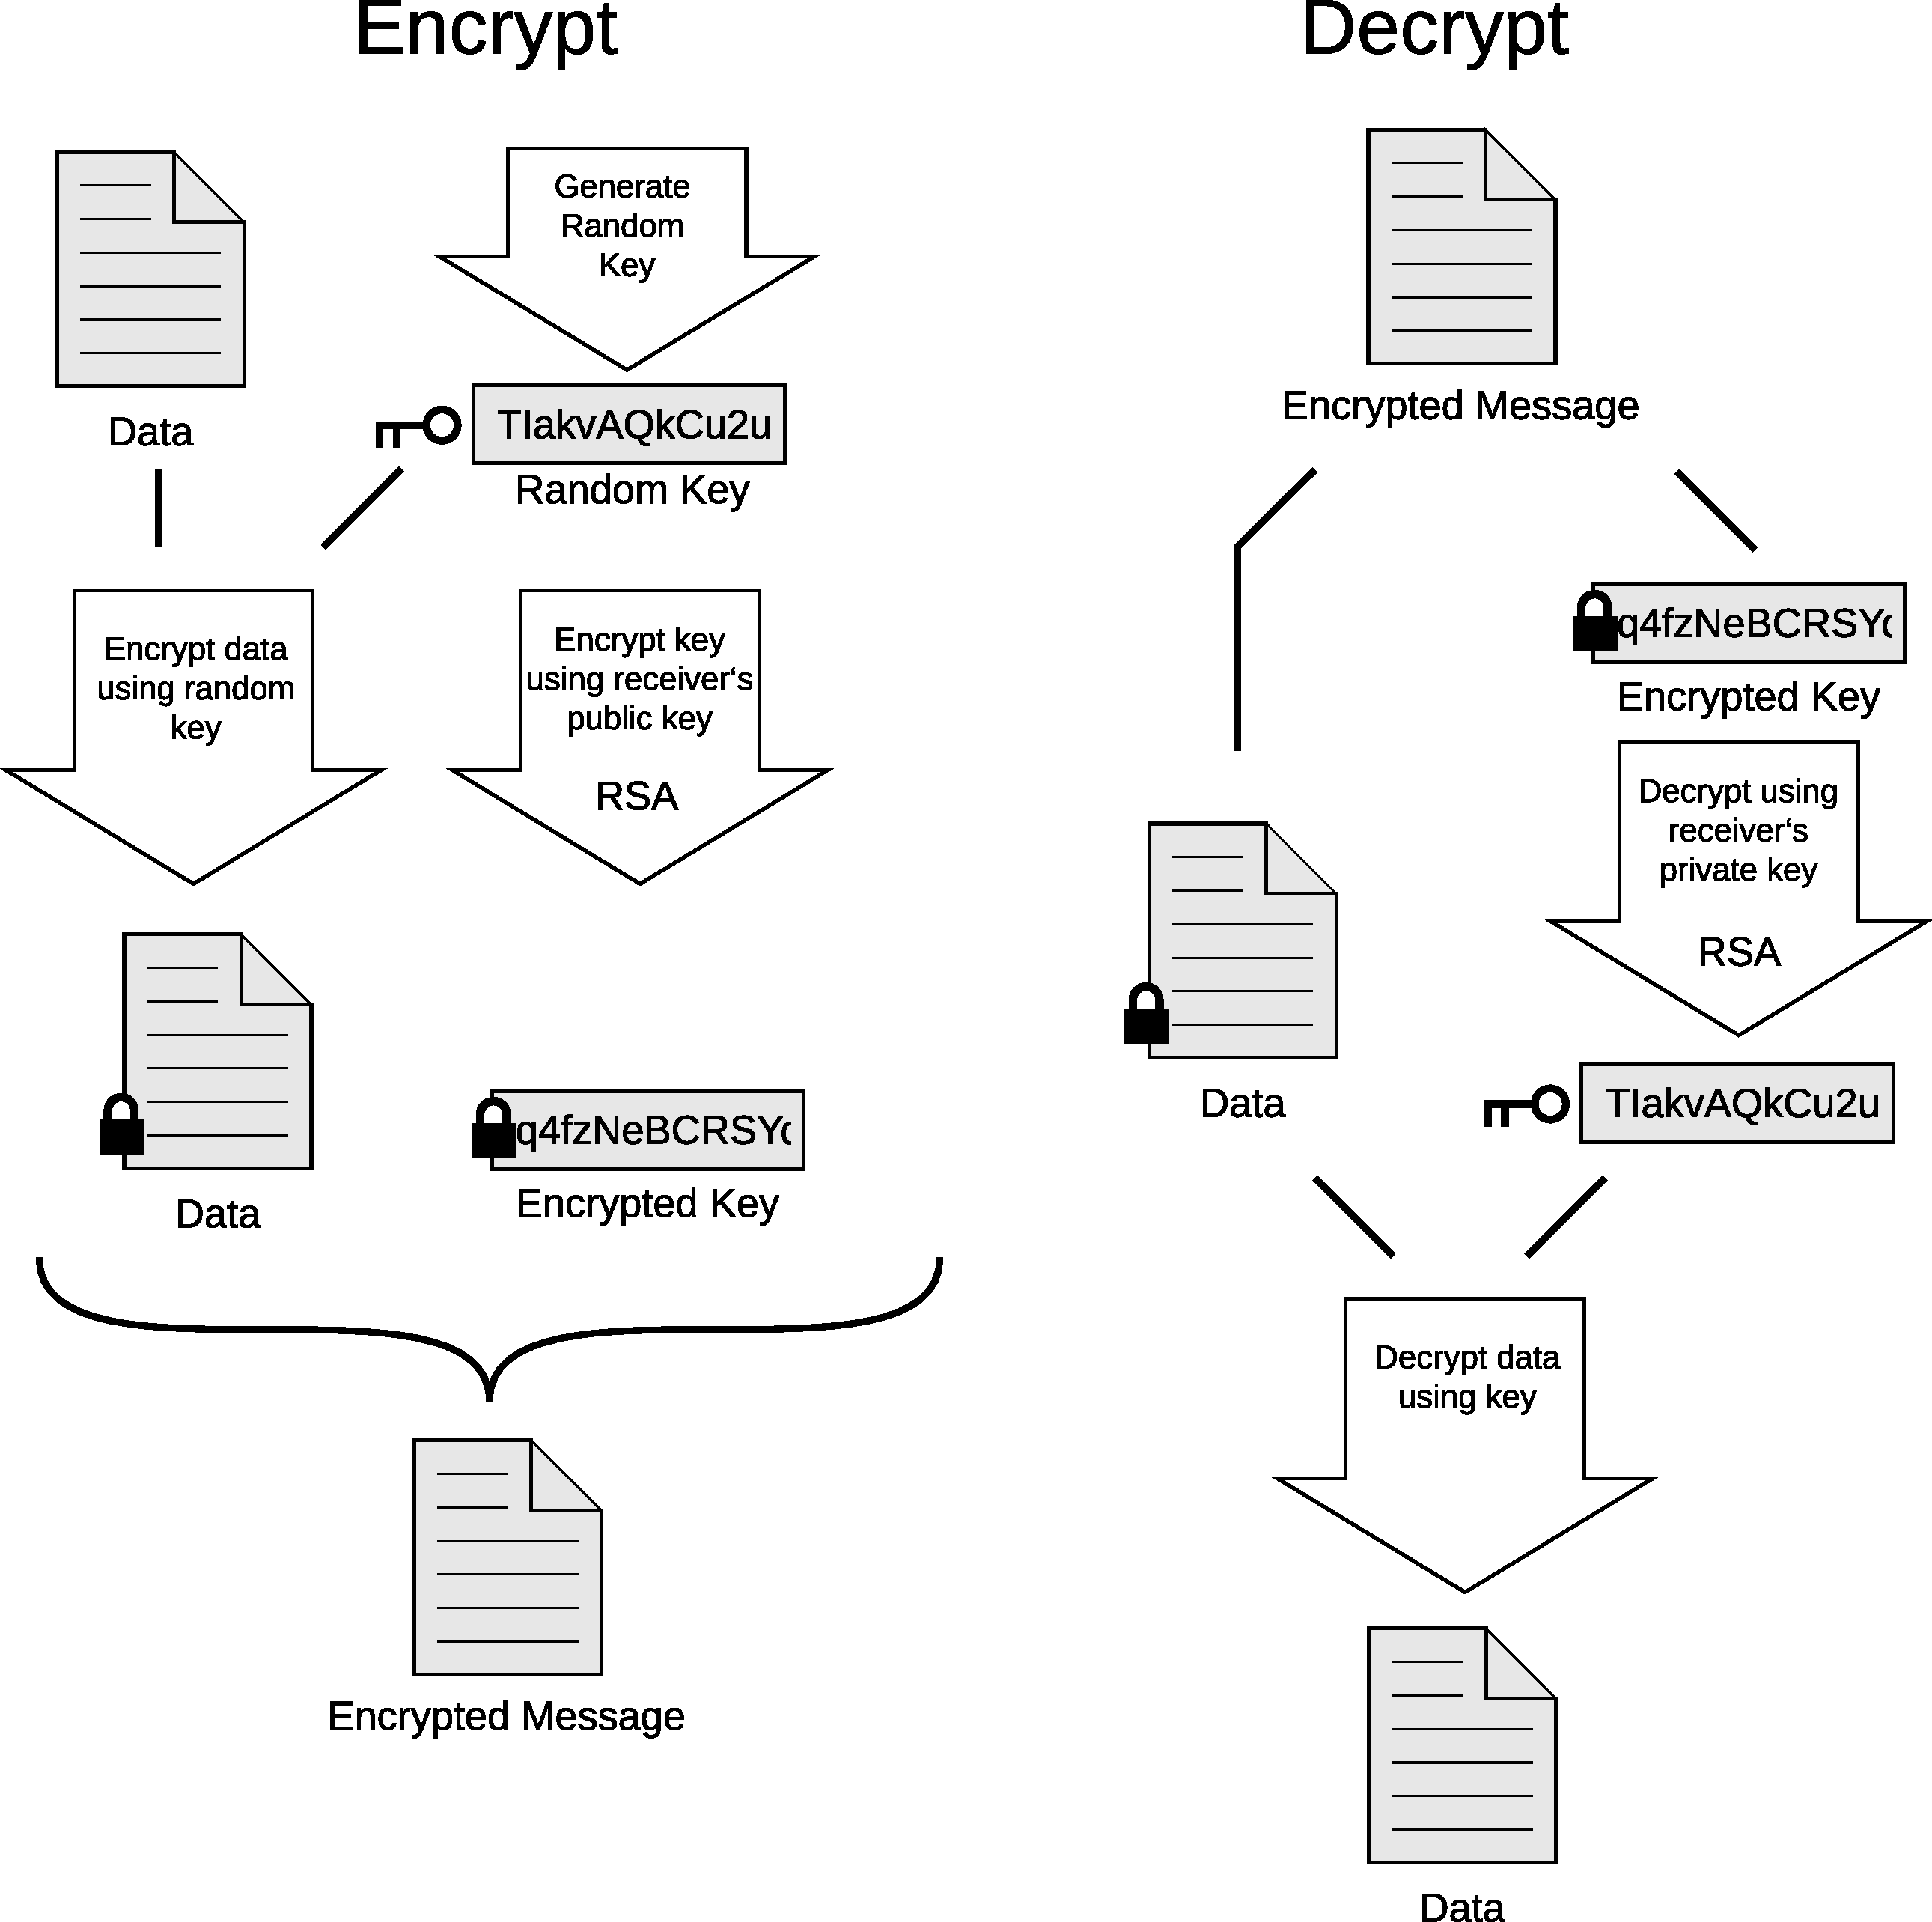
\includegraphics[width=0.7\linewidth]{graphics/PGP_diagram.pdf}
    \end{center}
\end{frame}

\begin{frame}
    \frametitle{GNU Privacy Guard}
    
\includegraphics[width=3cm]{graphics/Gnupg_logo.pdf}
    \begin{itemize}[<+->]
        \item Free implementation of OpenPGP standard
        \item Typically interfaced through \texttt{gpg} command line tool, but
            various GUI's are available
        \item Probably already on your system as most package managers
            (\texttt{pacman}, \texttt{apt}, etc) require it for package
            verification
        \item See \texttt{man gpg} for all of its options
    \end{itemize}
\end{frame}

\begin{frame}
    \frametitle{Web of Trust}
    How can I trust PGP content someone sends me?
    \pause
    \begin{block}{Phil Zimmermann, PGP creator}
        \small \itshape
        As time goes on, you will accumulate keys from other people that you
        may want to designate as trusted introducers. Everyone else will each
        choose their own trusted introducers. And everyone will gradually
        accumulate and distribute with their key a collection of certifying
        signatures from other people, with the expectation that anyone
        receiving it will trust at least one or two of the signatures. This
        will cause the emergence of a decentralized fault-tolerant web of
        confidence for all public keys.
    \end{block}
    \pause
    \begin{itemize}[<+->]
        \item Meet with them in person and verify the key fingerprints match,
            then sign their key.
        \item Or, verify someone you trust has signed their key.
    \end{itemize}
\end{frame}

\begin{frame}
    \frametitle{Making your own PGP key}
    \begin{enumerate}[<+->]
        \item \texttt{\$ gpg --gen-key}
        \item \texttt{gpg} will ask you a number of questions... answer them
        \item After making a secure passphrase, you will have to wait a few
            minutes for it to generate a key. During this time, you may want to
            browse the web, or do something else to increase system entropy, as
            this will speed up the prime number generation.
        \item \texttt{\$ gpg --list-keys} and make sure your new key is there
        \item Upload your key to a keyserver like \texttt{pgp.mit.edu}\par
            \texttt{\small \$ gpg --keyserver pgp.mit.edu --send-keys \emph{B20E73F7}}
    \end{enumerate}
\end{frame}

\begin{frame}
    \frametitle{Generating a Revocation Certificate}
        \begin{enumerate}[<+->]
            \item \texttt{\$ gpg --output revoke.asc --gen-revoke \emph{B20E73F7}}
            \item ``If you forget your passphrase or if your private key is compromised or lost, this revocation certificate may be published to
                notify others that the public key should no longer be used.''
            \item Revoked public keys:
                \begin{enumerate}
                    \item can still verify signatures made by you in the past
                    \item cannot be used to encrypt future messages to you
                    \item do not affect ability to decrypt previously received messages (because that depends on your private key)
                \end{enumerate}
            \item Store a physical (e.g., printed) copy of the revocation certificate in a lock box
        \end{enumerate}
        \visible<7>{
            \begin{center}
                
\includegraphics[width=0.4\linewidth]{graphics/gandalf.png}
            \end{center}
        }
\end{frame}

\begin{frame}
    \frametitle{Signing others' keys}
    \begin{enumerate}[<+->]
        \item Get their key from a keyserver\par
            \texttt{\small \$ gpg --keyserver pgp.mit.edu --recv \emph{B20E73F7}}
        \item \texttt{\$ gpg --sign-key \emph{B20E73F7}}
        \item Have them run \texttt{\$ gpg --fingerprint} in person and verify
            the fingerprint matches the one on your terminal
        \item Send their key (now signed) back to the keyserver.\par
            \texttt{\small \$ gpg --keyserver pgp.mit.edu --send-keys \emph{B20E73F7}}
    \end{enumerate}
\end{frame}

\begin{frame}
    \frametitle{Integrating GnuPG with your email client}
    \begin{itemize}
        \item Thunderbird: Install the Enigmail addon. The GUI is pretty self
            explanatory.
        \item Mutt: See \texttt{http://dev.mutt.org/trac/wiki/MuttGuide/UseGPG}
        \item Android: Use K9 mail and install APG
        \item Other email clients: Google it
    \end{itemize}
    When setting up your email client, please use PGP/MIME, as
    \emph{inline PGP is considered harmful}.
\end{frame}


\end{document}
